\documentclass[a4paper]{article}
\usepackage{import}
%\usepackage[english,vietnam]{babel}
\usepackage[utf8]{inputenc}
%\usepackage[utf8]{inputenc}
%\usepackage[francais]{babel}
\usepackage{a4wide,amssymb,epsfig,latexsym,array,hhline,fancyhdr}
\usepackage[normalem]{ulem}
%\usepackage{soul}
\usepackage{listings}
\usepackage{colortbl}
\usepackage[makeroom]{cancel}
\usepackage{amsmath}
\usepackage{amsthm}
\usepackage{multicol,longtable,amscd}
\usepackage{diagbox}%Make diagonal lines in tables
\usepackage{booktabs}
\usepackage{alltt}
\usepackage[framemethod=tikz]{mdframed}% For highlighting paragraph backgrounds
\usepackage{caption,subcaption}

\usepackage{lastpage}
\usepackage[lined,boxed,commentsnumbered]{algorithm2e}
\usepackage{enumerate}
\usepackage{color}
\usepackage{graphicx}							% Standard graphics package
\usepackage{array}
\usepackage{tabularx, caption}
\usepackage{multirow}
\usepackage{multicol}
\usepackage{rotating}
\usepackage{graphics}
\usepackage{geometry}
\usepackage{setspace}
\usepackage{epsfig}
\usepackage{minted}
\usepackage{xcolor} % to access the named colour LightGray
\definecolor{LightGray}{gray}{0.9}
\usemintedstyle{emacs}
\usepackage{tikz}
\usetikzlibrary{graphs,graphs.standard}
\usetikzlibrary{arrows,snakes,backgrounds}
\usepackage[unicode]{hyperref}
\hypersetup{
    urlcolor=blue,
    linkcolor=black,
    citecolor=black,
    colorlinks=true,
    pdfpagemode=FullScreen,
    pdftitle={The Travelling Salesman Problem},
} 
%\usepackage{pstcol} 								% PSTricks with the standard color package
%\usepackage{background}
%\backgroundsetup{contents=
\includegraphics{Images/hcmut.png}, scale=0.5, opacity=0.25, angle = 0}
\usepackage[normalem]{ulem}

\def\thesislayout{	% A4: 210 × 297
	\geometry{
		a4paper,
		total={160mm,240mm},  % fix over page
		left=30mm,
		top=30mm,
	}
}
\thesislayout

\usepackage{fancyhdr}
\setlength{\headheight}{40pt}
\pagestyle{fancy}
\fancyhead{} % clear all header fields
\fancyhead[L]{
 \begin{tabular}{rl}
    \begin{picture}(25,15)(0,0)
    \put(0,-8){
\includegraphics[width=8mm, height=8mm]{Images/hcmut.png}}
    %\put(0,-8){\epsfig{width=10mm,figure=hcmut.eps}}
   \end{picture}&
	%
\includegraphics[width=8mm, height=8mm]{hcmut.png} & %
	\begin{tabular}{l}
		\textbf{\textcolor{blue}{\bf \ttfamily Ho Chi Minh City University of Technology}}\\
		\textbf{\textcolor{blue}{\bf \ttfamily Faculty of Computer Science and Engineering}}
	\end{tabular} 	
 \end{tabular}
}
\fancyhead[R]{
	\begin{tabular}{l}
		\tiny \bf \\
		\tiny \bf 
	\end{tabular}  }
\fancyfoot{} % clear all footer fields
\fancyfoot[L]{\scriptsize \ttfamily Truong Gia Ky Nam - 2352787}
\fancyfoot[R]{\scriptsize \ttfamily Page {\thepage}/\pageref{LastPage}}
\renewcommand{\headrulewidth}{0.3pt}
\renewcommand{\footrulewidth}{0.3pt}


%%%
\setcounter{secnumdepth}{4}
\setcounter{tocdepth}{3}
\makeatletter
\newcounter {subsubsubsection}[subsubsection]
\renewcommand\thesubsubsubsection{\thesubsubsection .\@alph\c@subsubsubsection}
\newcommand\subsubsubsection{\@startsection{subsubsubsection}{4}{\z@}%
                                     {-3.25ex\@plus -1ex \@minus -.2ex}%
                                     {1.5ex \@plus .2ex}%
                                     {\normalfont\normalsize\bfseries}}
\newcommand*\l@subsubsubsection{\@dottedtocline{3}{10.0em}{4.1em}}
\newcommand*{\subsubsubsectionmark}[1]{}
\makeatother

\sloppy
\captionsetup[figure]{labelfont={small,bf},textfont={small,it},belowskip=-1pt,aboveskip=-9pt}
%space remove between caption, figure, and text
\captionsetup[table]{labelfont={small,bf},textfont={small,it},belowskip=-1pt,aboveskip=7pt}
%space remove between caption, table, and text

%\floatplacement{figure}{H}%forced here float placement automatically for figures
%\floatplacement{table}{H}%forced here float placement automatically for table
%the following settings (11 lines) are to remove white space before or after the figures and tables
%\setcounter{topnumber}{2}
%\setcounter{bottomnumber}{2}
%\setcounter{totalnumber}{4}
%\renewcommand{\topfraction}{0.85}
%\renewcommand{\bottomfraction}{0.85}
%\renewcommand{\textfraction}{0.15}
%\renewcommand{\floatpagefraction}{0.8}
%\renewcommand{\textfraction}{0.1}
\setlength{\floatsep}{5pt plus 2pt minus 2pt}
\setlength{\textfloatsep}{5pt plus 2pt minus 2pt}
\setlength{\intextsep}{10pt plus 2pt minus 2pt}

\thesislayout



\begin{document}
\begin{titlepage}
\begin{center}
\textbf{\Large VIETNAM NATIONAL UNIVERSITY HO CHI MINH CITY} \\

\vspace{7pt}
\textbf{\Large HO CHI MINH CITY UNIVERSITY OF TECHNOLOGY} \\

\vspace{7pt}
\textbf{\Large FACULTY OF COMPUTER SCIENCE AND ENGINEERING}
\end{center}

\vspace{1cm}

\begin{figure}[h!]
\begin{center}

\includegraphics[width=3cm]{Images/hcmut.png}
\end{center}
\end{figure}

\vspace{1cm}


\begin{center}
\begin{tabular}{ccc}
	\multicolumn{3}{l}{\textbf{{\Large \textcolor{blue}{DISCRETE STRUCTURE}}}}\\
	~~\\
	\arrayrulecolor{blue}\hline
	\\
	\multicolumn{3}{l}{\textbf{{\Large \textcolor{blue}{Assignment 1} }}}\\
	\\
	
	\multicolumn{3}{c}{\textbf{{\huge \textcolor{blue}{Using Branch And Bound Algorithm}}}}\\
	\\
    
    \multicolumn{3}{c}{\textbf{{\huge \textcolor{blue}{To Solve The Travelling Saleman Problem}}}}\\
	\\
	\arrayrulecolor{blue}\hline \\ \\

    \multicolumn{1}{r}{\textbf{\Large Instructors:}} & \multicolumn{2}{l}{\Large Nguyen Van Minh Man, \textit{Mahidol University}} \\ \\
    \multicolumn{1}{r}{} & \multicolumn{2}{l}{\Large Tran Tuan Anh, \textit{CSE-HCMUT}} \\ \\

    \\ \\

    \multicolumn{1}{r}{\Large \textbf{Author:}} & \multicolumn{2}{l}{\Large Truong Gia Ky Nam} \\ \\

    \multicolumn{1}{r}{\Large \textbf{ID:}} & \multicolumn{2}{l}{\Large 2352787} \\ \\

    \multicolumn{1}{r}{\Large \textbf{Email:}} & \multicolumn{2}{l}{\Large nam.truonggiaky@hcmut.edu.vn} \\ \\
\end{tabular}
\end{center}

\vspace{4cm}

\begin{center}
{\textbf{\Large Ho Chi Minh City, May 2024}}
\end{center}
\end{titlepage}

\thispagestyle{empty}
\setcounter{page}{-1}
\newpage
\begin{abstract}
    \noindent 
\end{abstract}
\newpage

\setcounter{page}{0}
\thispagestyle{empty}
\newpage
\tableofcontents
\newpage

%\thispagestyle{empty}
\section{Introduction}
This report aims to provide a comprehensive explaination of The Traveling Salemen Problem along with the Branch and Bound algorithm. By delving into the Branch and Bound algorithm and implement it using the C++ language, this report seek to highlights its effectiveness in solving one of the most challenging problems in optmization. 
\section{The Traveling Salemen Problem}
\subsection{Overview}
The Travelling Salesman Problem, also known as The Travelling Salesperson Problem (TSP), asks the following question: \textit{``Given a list of cities and the distances between each pair of cities, what is the shortest possible route that visits each city exactly once and returns to the origin city?"} or in other words, the problem is: \textit{``Given a complete graph with weight edges, what is the Hamiltonian cycle of minimum cost?}. It is an NP-hard problem in combinatorial optimization, important in theoretical computer science and operations research.
\subsection{Traveling Saleman Problem implementation}
Although TSP is a problem in computer science, it has a wide range of applications in various fields:
\begin{itemize}
    \item \textbf{Logistics and Supply Chain Managment}: TSP can determine the most efficient routes for delivery transportation, reducing travel time and fuel consumption,which can help the companies to save lots of money.
    \item \textbf{Manufacturing}: In manaufacturing processes involving CNC machines, TSP helps in determining the optimal path for tools, reducing the time and cost of production.
    \item \textbf{Transportation}: TSP can help public transport such as buses or trains to minimize travel time and improve service efficiency.
    \item \textbf{Telecommunications}: TSP is used in the design of efficient telecommunication networks, ensuring that the data transmission routes are optimized to reduce latency and cost.
\end{itemize}
By solving the TSP, we can address real-world challenges more effectively, leading to substantial economic, operational, and environmental benefits.
\subsection{Traveling Saleman Problem solving methods}
Throught out the history, many methods have been made to find the optimal solution for TSP:
\begin{itemize}
    \item \textbf{Brute-Force Search}: This is the straight-forward solution by computing all possible permutations of the cities until the shortest path is found.
    \item \textbf{Nearest Neighbor Algorithms}: Start from the origin city, repeatedly visit the nearest unvisited city until all cities are visited.
    \item \textbf{Held-Karp Algorithm}: This approach using dynamic programming to solve TSP. It is more efficient than brute force but still exponential.  
    \item \textbf{Christofides's Algorithm}: This algorithm involves constructing a minimum spanning tree, finding a minimum matching, and combining these to form a tour. 
    \item \textbf{Genetic Algorithms}:These use principles of natural selection and genetics to evolve a population of solutions over several generations, aiming to improve the quality of solutions.
\end{itemize}
And there are others algorithm and heuristics which can be used to solve TSP. Each method has its advantages and disadvantages, depending on the problem size, required solution quality, and computational resources. In my report, I will focusing on solving TSP using the \textbf{Branch and Bound} algorithm, a well used algorithm for optmization problems.   
\section{Branch and Bound Algorithm}
\subsection{Overview}
Branch and bound is a method used in computer science to solve optimization problems. Branch and bound algorithms involves dividing the problem space into smaller sub-problems and applying constraints or bounds to eliminate certain sub-problems. This process continue until the optimal solution is found.
\subsection{Some basic concepts}
Before getting into the algorithms, first I need to declare some basic concepts:
\begin{itemize}
    \item \textbf{Branching}: This is the process where the big problem are divided into smaller subproblems (branches) that easy to solve.
    \item \textbf{Bounding}: Calculating the lower bound (for minimization problems) or an upper bound (for maximization problems) on the optimal solution within a branch.
    \item \textbf{Pruning}: ``Cutting'' the branches that can not yield a better solution than the current best-known solution.
    \item \textbf{Search Tree}: The structure used to represent the branching of subproblems. Each node in the tree represents a subproblem.
    \item \textbf{Backtracking}: Return to the previous node to explore other branches after completing the exploration of a branch 
\end{itemize}
\subsection{Applications of Branch and Bound}
Beside solving TSP, Branch and Bound algorithm has many applications. It includes:
\begin{itemize}
    \item \textbf{Solving Knapsack Problem}: Branch and Bound is used to solve the Knapsack Problem, which involves finding the optimized combination of items to pack into a knapsack of limited capacity.
    \item \textbf{Resource Allocation}: Branch and Bound is used to solve resource allocation problems, like scheduling work on machines or assigning work to workers. 
    \item \textbf{Network Optimization}: Branch and bound is used to solve network optimization problems, it helps in finding the optimized path or flow through a network.
    \item \textbf{Game Playing}: Branch and bound is used in some of the game-playing algorithms, like chess or tic-tac or 16 puzzle problem, to explore the various possible moves and find the optimized strategies.
\end{itemize}
\subsection{Advantages and Disadvantages}
There are advantages when using this algorithms:
\begin{itemize}
    \item By pruning the search space using bounds, it can avoid exploring irrelevant sub-problems and find the optimal solution more quickly when compare to other algorithms.
    \item There is a guarantees that the optimal solution will be found, as long as the bounds are computed correctly. This makes it a reliable algorithm for solving optimization problems.
    \item Branch and bound can be applied to a wide range of optimization problems, including linear programming, integer programming, and combinatorial optimization problems.
    \item  Branch and bound can be used to solve large-scale optimization problems, as it can be parallelized and distributed across multiple processors.
\end{itemize}
However, there are some drawbacks when using Branch and Bound algorithms
\begin{itemize}
    \item Branch and bound can be a complex algorithm to implement, as it requires careful design of the bounds and branching strategy.
    \item The performance of branch and bound is highly dependent on the quality of the bounds used. If the bounds are too loose, the algorithm may explore too many irrelevant sub-problems, leading to poor performance.
\end{itemize}
\section{Detailed Explanation of the Algorithm}
\subsection{Initialization}
\subsection{Branching}
\subsection{Bounding}
To use the Branch and Bound algorithms, first we need to compute the bound (in TSP is the lower bound) on the best solution. We can find the bound of any path by the following idea:\\ \\
For any tour T, the cost of any tour can be written as:
\begin{center}
    Tour cost = $\frac{1}{2}$ $\times$ (Sum of cost of two edges adjacent to u and in the tour T) 
\end{center}
Because for every vertex u, there are two edges through it in T
and sum their costs. The overall sum for all vertices would
be twice of cost of tour T.\\ \\
For a clearer explaination, I will create an small example of TSP with 4 cities
\begin{center}
    \tikzset{every picture/.style={line width=0.75pt}} %set default line width to 0.75pt        

    \begin{tikzpicture}[x=0.75pt,y=0.75pt,yscale=-1,xscale=1]
    %uncomment if require: \path (0,336); %set diagram left start at 0, and has height of 336
    
    %Shape: Circle [id:dp8852483719720448] 
    \draw   (205,70) .. controls (205,56.19) and (216.19,45) .. (230,45) .. controls (243.81,45) and (255,56.19) .. (255,70) .. controls (255,83.81) and (243.81,95) .. (230,95) .. controls (216.19,95) and (205,83.81) .. (205,70) -- cycle ;
    %Shape: Circle [id:dp9765888742621183] 
    \draw   (376,70) .. controls (376,56.19) and (387.19,45) .. (401,45) .. controls (414.81,45) and (426,56.19) .. (426,70) .. controls (426,83.81) and (414.81,95) .. (401,95) .. controls (387.19,95) and (376,83.81) .. (376,70) -- cycle ;
    %Shape: Circle [id:dp1060732376012139] 
    \draw   (206,165) .. controls (206,151.19) and (217.19,140) .. (231,140) .. controls (244.81,140) and (256,151.19) .. (256,165) .. controls (256,178.81) and (244.81,190) .. (231,190) .. controls (217.19,190) and (206,178.81) .. (206,165) -- cycle ;
    %Shape: Circle [id:dp7781749612954871] 
    \draw   (377,165) .. controls (377,151.19) and (388.19,140) .. (402,140) .. controls (415.81,140) and (427,151.19) .. (427,165) .. controls (427,178.81) and (415.81,190) .. (402,190) .. controls (388.19,190) and (377,178.81) .. (377,165) -- cycle ;
    %Straight Lines [id:da13303541362906368] 
    \draw    (255,70) -- (376,70) ;
    %Straight Lines [id:da7085298181670543] 
    \draw    (230,95) -- (231,140) ;
    %Straight Lines [id:da15835860667428836] 
    \draw    (401,95) -- (402,140) ;
    %Straight Lines [id:da004405079700216641] 
    \draw    (250,85.27) -- (380.33,151.27) ;
    %Straight Lines [id:da7901368293801847] 
    \draw    (382,86.27) -- (254.33,153.27) ;
    %Straight Lines [id:da7094591705832543] 
    \draw    (256,165) -- (377,165) ;
    
    % Text Node
    \draw (225,156.27) node [anchor=north west][inner sep=0.75pt]   [align=left] {B};
    % Text Node
    \draw (396,155.27) node [anchor=north west][inner sep=0.75pt]   [align=left] {C};
    % Text Node
    \draw (224,61.27) node [anchor=north west][inner sep=0.75pt]   [align=left] {D};
    % Text Node
    \draw (396,61.27) node [anchor=north west][inner sep=0.75pt]   [align=left] {A};
    % Text Node
    \draw (307,52) node [anchor=north west][inner sep=0.75pt]   [align=left] {15};
    % Text Node
    \draw (216,109.27) node [anchor=north west][inner sep=0.75pt]   [align=left] {5};
    % Text Node
    \draw (403,113.27) node [anchor=north west][inner sep=0.75pt]   [align=left] {7};
    % Text Node
    \draw (312,167.27) node [anchor=north west][inner sep=0.75pt]   [align=left] {13};
    % Text Node
    \draw (349.8,115.98) node [anchor=north west][inner sep=0.75pt]  [rotate=-27.97] [align=left] {20};
    % Text Node
    \draw (278.36,120.19) node [anchor=north west][inner sep=0.75pt]  [rotate=-333.2] [align=left] {22};
    
    \end{tikzpicture}
\end{center}
Consider the tour $T_1$: A - C - D - B - A, the toal cost of this tour is:
\begin{equation*}
    T_1 = 7 + 20 + 5 + 22 = 54
\end{equation*}
In tour $T_1$, the edges that adjacent to vertex A have the weight 7 and 22. Similarly for vertex B are 22 and 5; vertex C are 20 and 7; vertex D are 5 and 20. Using the above idea:
\begin{equation*}
    T_1 = \frac{1}{2} \times (7 + 22 + 22 + 5 + 20 + 7 + 5 + 20) = 54
\end{equation*}
Or consider tour $T_2$: B - C - A - D - B, the total cost of this tour is: 
\begin{equation*}
    T_2 = 13 + 7 + 15 + 5 = 40
\end{equation*}
In tour $T_2$, the edges that adjacent to vertex B have the weight 13 and 5. Similarly for vertex C is 13 and 7; vertex A is 15 and 7; vertex D is 5 and 15. Using the above idea:
\begin{equation*}
    T_2 = \frac{1}{2} \times (13 + 5 + 13 + 7 + 15 + 7 + 15 + 5) = 40
\end{equation*}
For every vertex in the graph, we have:
\begin{center}
    (Sum of two tour edges adjacent to u) $\geqslant$ (Sum of minimum weight two edges adjacent to u)   
\end{center}
From that, we have:
\begin{center}
    Cost any tour $\geqslant$ $\frac{1}{2}$ $\times$  (Sum of minimum weight two edges adjacent to u)
\end{center}
Consider the above graph, we have:
\begin{center}
    \begin{tabular}{|c|c|c|}
        \hline
        Node & Minimum cost edges & Total cost\\
        \hline
        A & (A,D);(A,C) & 22 \\
        \hline
        B & (B,D);(B,C) & 18 \\
        \hline
        C & (C,B);(C,A) & 20 \\
        \hline
        D & (D,B);(D,A) & 20 \\
        \hline
    \end{tabular}
\end{center}
The lower bound of the cost of any tour in the given graph is:
\begin{equation*}
    t = \frac{1}{2} \times (22 + 18 + 20 + 20) = 40
\end{equation*} 
So now we need functions find the first and second minimum edge cost having an end at vertex u to calculate the lower bound of any node
\subsection{Pruning}
\subsection{Termination}

\section{Implementation Details} % Make 2-3 testcase and implement it
\section{Complexity Analysis} % Time and space complexity
The Branch and Bound algorithm for solving the Traveling Salesman Problem (TSP) can be analyzed in terms of both time and space complexity.
\subsection{Time Complexity}
The time complexity of Branch and Bound algorithm to solving TSP is analyze as below
\begin{itemize}
    \item Finding two minimum values for each city requires $O(n^2)$ time in total (each call to `findTwoMin' function is $O(n)$, and it's called $n$ times)
    \item In the worst-case scenario, the time complexity is $O(n!)$ where n is the number of cities. This is because the algorithm have to explore all permutations of cities. However, due to the pruning procedure, the real performance is much better.
    \item Each node exploration in the search tree involves computing the bound and making decisions based on the bound, which is $O(n)$
\end{itemize}
Overall, the worst-case time complexity is factorial term $O(n!)$ but with effective pruning technique, the performance is often better. 
\subsection{Space complexity}


\section{Experimental Results}
\section{Challenges and Improvements} % Method to get Bound
\section{Conclusion}

\begin{minted}[
frame=lines,
framesep=2mm,
baselinestretch=1.2,
fontsize=\footnotesize,
linenos
]{cpp}
void findTwoMin(int G[20][20], int numCities, int i, int &first, int &second)
{
    first = INT_MAX, second = INT_MAX;
    for (int j = 0; j < numCities; j++)
    {
        if (i == j)
            continue;
        if (G[i][j] <= first)
        {
            second = first;
            first = G[i][j];
        }
        else if (G[i][j] <= second && G[i][j] != first)
        {
            second = G[i][j];
        }
    }
}
\end{minted}

\begin{minted}[
    frame=lines,
    framesep=2mm,
    baselinestretch=1.2,
    fontsize=\footnotesize,
    linenos
    ]{cpp}
void branchAndBoundTSP(int G[20][20], int numCities, int (&curr_path)[21], int &curr_bound, 
int curr_weight, int level, bool (&visited)[20], int &min_cost, int (&final_path)[21])
{
    if (level == numCities)
    {
        if (G[curr_path[level - 1]][curr_path[0]] != 0)
        {
            int curr_res = curr_weight +
                           G[curr_path[level - 1]][curr_path[0]];

            if (curr_res < min_cost)
            {
                for (int i = 0; i < numCities; i++)
                {
                    final_path[i] = curr_path[i];
                }
                final_path[numCities] = curr_path[0];
                min_cost = curr_res;
            }
        }
    }
    else
    {
        for (int i = 0; i < numCities; i++)
        {
            if (G[curr_path[level - 1]][i] != 0 &&
                visited[i] == false)
            {
                int temp = curr_bound;
                curr_weight += G[curr_path[level - 1]][i];

                int firstMinCurr, secondMinCurr;
                findTwoMin(G, numCities, curr_path[level - 1], firstMinCurr, secondMinCurr);
                int firstMinNext, secondMinNext;
                findTwoMin(G, numCities, i, firstMinNext, secondMinNext);

                curr_bound -= ((secondMinCurr + firstMinNext) / 2);

                // curr_bound -= ((secondMin(G, numCities, curr_path[level - 1]) + firstMin(G, numCities, i)) / 2);

                if (curr_bound + curr_weight < min_cost)
                {
                    curr_path[level] = i;
                    visited[i] = true;

                    branchAndBoundTSP(G, numCities, curr_path, curr_bound, curr_weight, level + 1, visited, min_cost, final_path);
                }

                curr_weight -= G[curr_path[level - 1]][i];
                curr_bound = temp;

                for (int i = 0; i < numCities + 1; i++)
                {
                    visited[i] = false;
                }

                for (int j = 0; j <= level - 1; j++)
                {
                    visited[curr_path[j]] = true;
                }
            }
        }
    }
}
\end{minted}

\begin{minted}[
    frame=lines,
    framesep=2mm,
    baselinestretch=1.2,
    fontsize=\footnotesize,
    linenos
    ]{cpp}
string Traveling(int G[20][20], int numCities, char startVertex)
{

    int curr_path[21] = {-1};
    bool visited[20] = {false};
    int final_path[21] = {-1};
    int min_cost = INT_MAX;
    int curr_bound = 0;
    string ans;

    for (int i = 0; i < numCities; i++)
    {
        int first, second;
        findTwoMin(G, numCities, i, first, second);
        curr_bound += (first + second);
        // curr_bound += (firstMin(G,numCities,i) + secondMin(G,numCities,i));
    }

    if (curr_bound % 2 == 0)
    {
        curr_bound = curr_bound / 2;
    }
    else
    {
        curr_bound = curr_bound / 2 + 1;
    }

    visited[int(startVertex - 'A')] = true;
    curr_path[0] = int(startVertex - 'A');

    branchAndBoundTSP(G, numCities, curr_path, curr_bound, 0, 1, visited, min_cost, final_path);

    for (int i = 0; i <= numCities; i++)
    {
        ans += char(final_path[i] + 'A');
        ans += " ";
    }

    return ans;
}
\end{minted}
\begin{thebibliography}{80}

\bibitem{CVX}
CVX Introduction
``\textbf{link: http://cvxr.com/cvx/doc/intro.html/}'',
\textit{What is CVX}.

\end{thebibliography}
\end{document}

